\begin{figure}[H] 
	\begin{subfigure}[b]{0.5\linewidth}
		\centering
		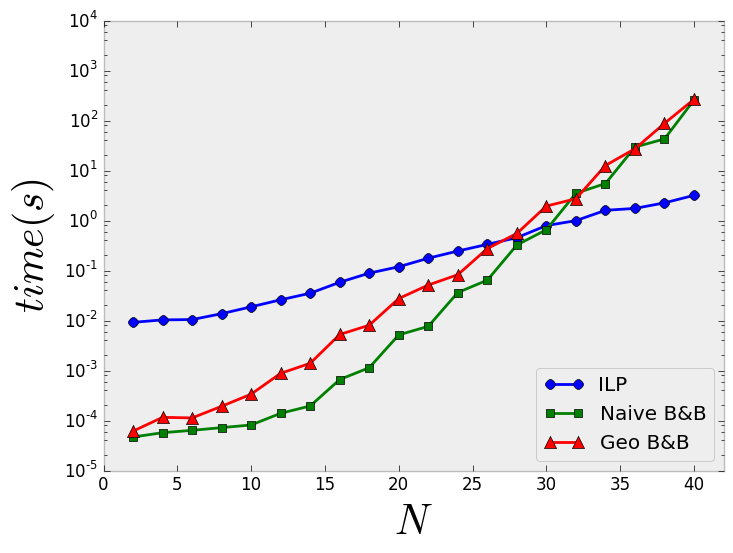
\includegraphics[width=0.9\linewidth]{Pictures/k1} 
		\caption{$K=0.25N$} 
		\label{fig:fixed_k:a} 
		\vspace{4ex}
	\end{subfigure}%% 
	\begin{subfigure}[b]{0.5\linewidth}
		\centering
		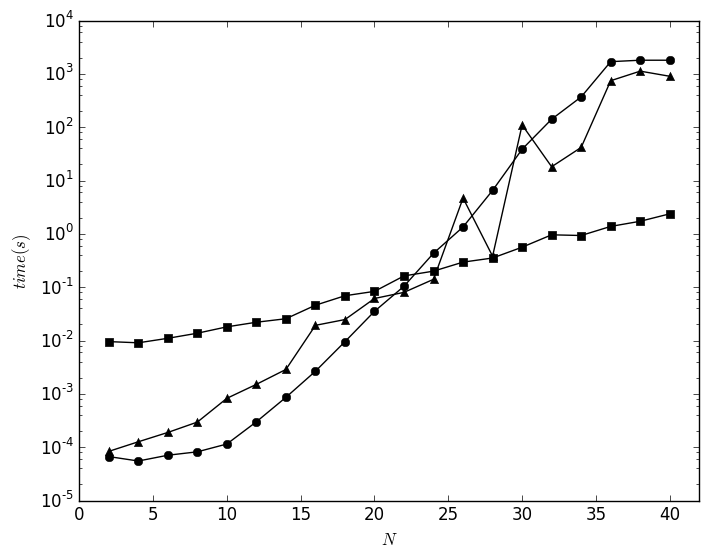
\includegraphics[width=0.9\linewidth]{Pictures/k2} 
		\caption{$K=0.5N$} 
		\label{fig:fixed_k:b} 
		\vspace{4ex}
	\end{subfigure} 
		\centering
		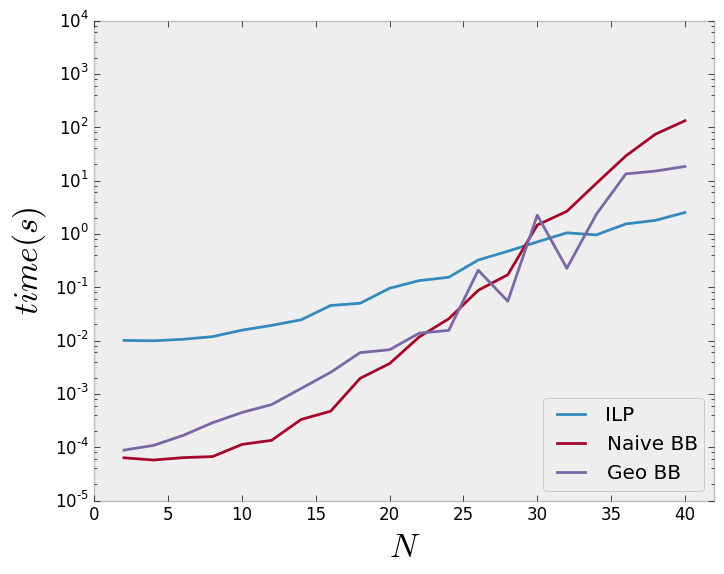
\includegraphics[width=0.45\linewidth]{Pictures/k3} 
		\caption{$K=0.75N$} 
		\label{fig:fixed_k:c} 
	\vspace{2ex}
	\smark\ -- Integer Linear Programming, \tmark\ -- Delaunay Assisted BB, \cmark\ -- Branch-and-bound
	\caption{Result times for different values of $K$ with varying values of $N$}
	\label{fig:fixed_k} 
\end{figure}

